% !TEX root = ../main.tex
\chapter{System Model}
\label{ch:systemmodel}

\begin{figure}[H]
    \centering
    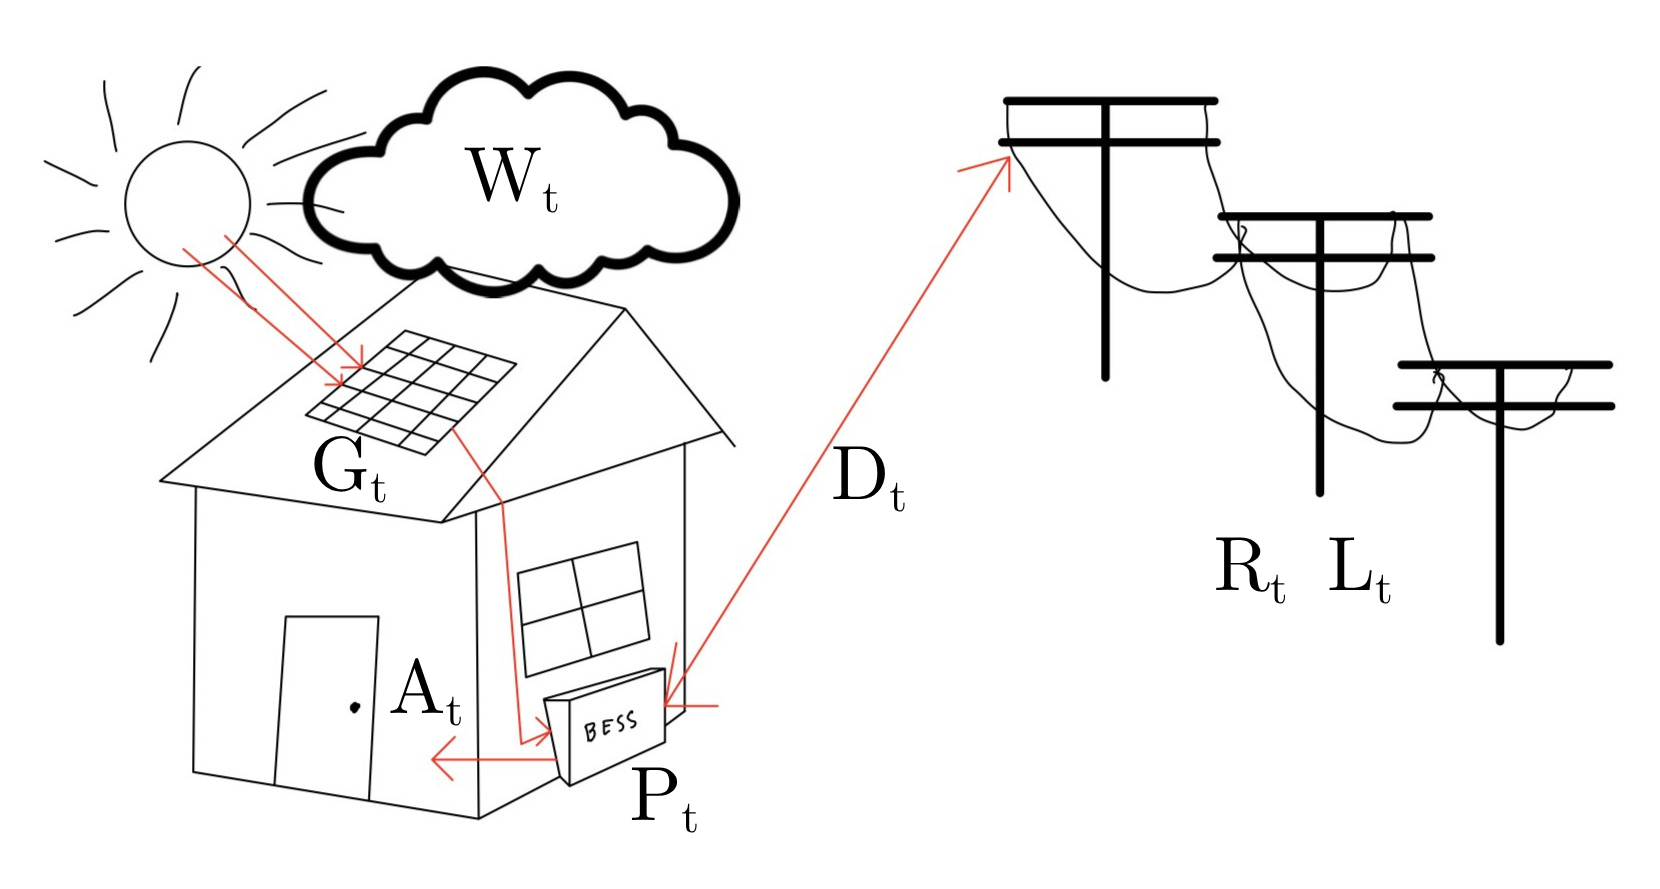
\includegraphics[width=0.8\textwidth]{images/sysmodel.png}
    \caption{A household with solar and batteries connected to the grid}
    \label{fig:sysmodel}
\end{figure}
Figure~\ref{fig:sysmodel} shows the basic system model that will be considered.

\section{Nomenclature}
\begin{description}
  \item[$W_t$] Weather variables $t$
  \item[$G_t$] Rooftop solar generation $t$ (kW) 
  \item[$A_t$] Household electricity consumption $t$ (kW)
  \item[$D_t^i$] Grid power imported (kW)
  \item[$D_t^e$] Grid power exported (kW)
    \item[$P_t^c$] Battery charging power $t$ (kW);
    \item[$P_t^d$] Battery discharging power $t$ (kW);
  \item[$E_t$] State of charge of battery $t$ (kWh)
  \item[$R_t$] NEM Regional Reference Price $t$ (\$/MWh)
  \item[$L_t$] Total demand in NEM region $t$ (MW)
  \item[$C^g_t$] Energy cost $t$ (\$)
    \item[$C^b_t$] Battery degradation cost $t$ (\$)
  \item[$\Delta t$] NEM dispatch period, 5 minutes
  \item[$N$] Network tariff (\$/kWh)
  \item[$P^c_{max}, P^d_{max}$] The maximum charging and discharging rates of the battery inverter (kW)
    \item[$E_{max}$] The maximum capacity of battery (kWh)
    \item[$E_{min}$] The minimum permitted state of charge (kWh), zero in this work because $E_{max}$ is the usable capacity
    \item[$E_0$] The state of charge at the start of the horizon (kWh)
    \item[$\eta^c$] Battery charging efficiency (\%)
    \item[$\eta^d$] Battery discharging efficiency (\%)
    \item[$\alpha_d$] Battery degradation coefficient (\$/kWh)
  \item[$J$] Number of cycle depth segments, indexed by $j$
  \item[$\delta$] Cycle depth, as a fraction of usable capacity
  \item[$\Phi(\delta)$] Cycle depth stress function (fraction of cell life lost per cycle of depth $\delta$)
  \item[$R^{\text{cell}}$] Battery replacement cost (\$)
  \item[$c_j$] Marginal aging cost of cycle depth segment $j$ (\$/kWh)
  \item[$E_j$] Energy capacity of cycle depth segment $j$ (kWh)
  \item[$P^{c}_{t,j}$] Battery charging power allocated to segment $j$ at $t$ (kW)
  \item[$P^{d}_{t,j}$] Battery discharging power allocated to segment $j$ at $t$ (kW)
  \item[$E_{t,j}$] Energy stored in cycle depth segment $j$ at $t$ (kWh)

\end{description}

\section{Objective}
The objective of the project is to minimise household expenditure on electricity consumption while considering battery degradation as defined in Equation~\ref{eq:goal}. This objective will be verified through simulations in Python using historical data.


\begin{equation}
    \label{eq:goal}
    \min \sum_{t=0}^{T} C^g_t+C^b_t
\end{equation}

\subsection{Cost of Energy}
The cost of energy is determined by the wholesale price, quantity traded, and network tariff. Network tariffs are only charged on electricity imported from the grid. The cost of energy can be modelled through Equation~\ref{eq:goal:G}.
\begin{equation}
    \label{eq:goal:G}
    C^g_t = D^i_t(N+R_t)\Delta t - D_t^e R_t\Delta t
\end{equation}

\subsection{Battery Degradation}
\label{sec:degradation}
Modelling battery degradation accurately is a highly non-linear process \cite{model_lithium}. The dominant operational stress factor is cycle depth: a cell cycled shallowly sustains far more cycles, and delivers far more lifetime energy throughput, than the same cell cycled deeply \cite{model_lithium}. A degradation cost that is linear in energy throughput cannot represent this, because it charges the same amount for many shallow cycles as for one deep cycle of equal throughput.

Let $\Phi(\delta)$ denote the cycle depth stress function, giving the fraction of cell life consumed by one full cycle of depth $\delta \in [0,1]$. Following Xu et al. \cite{Xu2018}, $\Phi$ is approximated by a piecewise linear function of $J$ segments that evenly divide the cycle depth range. Prorating the battery replacement cost $R^{\text{cell}}$ over the life consumed by each segment gives the marginal aging cost of segment $j$:

\begin{equation}
    \label{eq:goal:cj}
    c_j = \frac{R^{\text{cell}}}{\eta^d E_{max}}J
    \left[ \Phi\!\left(\frac{j}{J}\right) - \Phi\!\left(\frac{j-1}{J}\right) \right]
\end{equation}

Because $\Phi$ is convex, $c_1 \leq c_2 \leq \dots \leq c_J$, so a deeper segment is never cheaper than a shallower one. This convexity is what allows the model to be solved as a linear program: the optimiser always discharges the cheapest available segment first, which reproduces the cycle depths that the rainflow counting algorithm would identify without requiring that algorithm inside the optimisation \cite{Xu2018}. Following \cite{Xu2018}, aging is attributed to the discharging half cycle only, on the basis that the energy charged and discharged over a day are almost identical; charging is therefore not separately penalised.

The degradation cost at $t$ is the cost of the discharge power drawn from each segment:

\begin{equation}
    \label{eq:goal:B}
    C^b_t = \sum_{j=1}^{J} c_j P^d_{t,j} \Delta t
\end{equation}

Setting $J=1$ recovers a single constant marginal cost $c_1 = \alpha_d$, which is the linear degradation model. The number of segments $J$ is therefore a fidelity parameter rather than a change of model, and the effect of degradation model fidelity on dispatch can be evaluated by varying $J$, as proposed in Section~\ref{sec:bess_only}.

\subsection{Objective Function}
The objective is to determine values for $P^c_{t,j}$ and $P^d_{t,j}$ as stated in Equation~\ref{eq:goal:comb}. The constraints are discussed in the following section.

\begin{align}
    \min_{P^c_{t,j},P^d_{t,j}} \quad & \sum_{t=0}^{T} \left[ D^i_t (N+R_t)\Delta t - D_t^e R_t\Delta t + \sum_{j=1}^{J} c_j P^d_{t,j} \Delta t \right] \label{eq:goal:comb}\\
    \text{s.t.} \quad & \eqref{eq:cons:batModel} \nonumber\\
                      & \eqref{eq:cons:unidirec} \nonumber\\
                      & \eqref{eq:cons:demand} \nonumber
\end{align}


\section{Constraints}

\subsection{Battery Storage Model}
The battery model introduces constraints to the system as outlined in Equation~\ref{eq:cons:batModel}. The battery state of charge (SoC) is described in Equation~\ref{eq:batModel:soc}. Battery efficiency is a non-linear characteristic of the battery, conditions and SoC. To reduce complexity, this project will initially model a fixed efficiency however there is scope to more accurately optimise the operation.

$u^c_t$ and $u^d_t$ are binary variables. If the battery is charging $u^c_t = 1$ otherwise $u^c_t = 0$, $u^d_t$ follows the same logic for battery discharge. These binary variables are introduced to prevent the model from charging and discharging the battery simultaneously as used in \cite{Cao2020}.

Constraints \ref{eq:batModel:charge} and \ref{eq:batModel:discharge} reflect the battery inverter limits for charging and discharging the battery, which are asymmetric for the Powerwall 3 (Table~\ref{tab:powerwall3_specs}). \ref{eq:batModel:bound} bounds the battery SoC.

To represent cycle depth, the battery energy is disaggregated across the $J$ cycle depth segments introduced in Section~\ref{sec:degradation}. Each segment $j$ holds its own energy level $E_{t,j}$, bounded by the segment capacity $E_j = E_{max}/J$, and the total charge and discharge power is the sum of the per-segment components, \eqref{eq:batModel:sumc} and \eqref{eq:batModel:sumd}. Tracking energy per segment, \eqref{eq:batModel:soc}, allows the current cycle depth to be identified: because the marginal cost curve is convex, the battery discharges from the shallowest available segment towards the deeper, more expensive ones \cite{Xu2018}. The aggregate SoC is $E_t = \sum_j E_{t,j}$.

Constraint \ref{eq:batModel:terminal} requires the battery to finish the horizon with at least the energy it started with. Without it the model would discharge the battery in the final intervals regardless of subsequent prices, an end-of-horizon artefact that would overstate revenue.

\begin{subequations}
\label{eq:cons:batModel}
  \begin{align}
      E_{t,j} = E_{t-1,j} + P^c_{t,j} \eta^c \Delta t
      - \frac{P^d_{t,j}}{\eta^d} \Delta t \label{eq:batModel:soc}\\
      P^c_t = \sum_{j=1}^{J} P^c_{t,j} \label{eq:batModel:sumc} \\
      P^d_t = \sum_{j=1}^{J} P^d_{t,j} \label{eq:batModel:sumd} \\
      0 \leq P^c_t \leq u^c_t P^c_{max} \label{eq:batModel:charge} \\
      0 \leq P^d_t \leq u^d_t P^d_{max} \label{eq:batModel:discharge}\\
      0 \leq u^c_t + u^d_t \leq 1 \\
      u^c_t, u^d_t \in \{0,1\} \\
      0 \leq E_{t,j} \leq E_j \label{eq:batModel:segbound} \\
      E_{min} \leq \sum_{j=1}^{J} E_{t,j} \leq E_{max} \label{eq:batModel:bound} \\
      \sum_{j=1}^{J} E_{0,j} = E_0  \label{eq:batModel:initial} \\
      \sum_{j=1}^{J} E_{T,j} \geq E_0  \label{eq:batModel:terminal}
  \end{align}
\end{subequations}

\subsection{Unidirectional Power Flow}
Solar generation and household consumption is restricted to unidirectional power transfer.

\begin{subequations}
    \label{eq:cons:unidirec}
    \begin{align}
        A_t \geq 0 \\
        G_t \geq 0
    \end{align}
\end{subequations}

\subsection{Meet Demand}
The constraint defined in Equation~\ref{eq:cons:demand} ensures that household demand is always met.
\begin{equation}
    \label{eq:cons:demand}
    A_t = P^d_t - P^c_t + G_t + D^i_t - D^e_t
\end{equation}

\subsection{Observable State Space}
In this project, the household uses a smart electricity meter. Smart meters record the net
household electricity consumption at 5-minute resolution, and the reading for each slot is
assumed to be available to the controller before the next slot begins. Therefore the net
household electricity consumption is available for all time-slots before slot $n$, however the values of $G$ and $A$ are not known.
Denote the net household electricity before battery as 
\begin{equation}
    H = G-A
\end{equation}
The electricity spot price, in contrast, is revealed to the market by AEMO at the beginning
of each time slot $n$. The regional system demand $L$ published by AEMO is likewise
available for all time-slots before slot $n$.

The charge and discharge decisions at slot $n$ are functions of the system observations
available at time-slot $n$, \eqref{eq:sysknowledge:state}, and the history of previous
charge/discharge decisions, \eqref{eq:sysknowledge:decision}.

\begin{subequations}
    \begin{align}
        \textbf{V}_n &= \begin{bmatrix}
            H_1 & H_2 & \cdots & H_{n-1} & \\
            L_{1} & L_2 & \cdots & L_{n-1} & \\
            R_{1} & R_2 & \cdots & R_{n-1} & R_{n}
        \end{bmatrix} \label{eq:sysknowledge:state}  \\
        \textbf{K}_n &= \begin{bmatrix}
            P^c_{1} & P^c_{2} & \cdots & P^c_{n-1} \\
            P^d_{1} & P^d_{2} & \cdots & P^d_{n-1}
        \end{bmatrix} \label{eq:sysknowledge:decision}
    \end{align}
\end{subequations}

The charge and discharge power at each time slot $n$ are determined by a policy
that maps the available system observations $\textbf{V}_n$ and prior decisions
$\textbf{K}_n$ to a dispatch decision:
\begin{subequations}
    \begin{align}
        P^d_n = f_{d,n} (\textbf{V}_n,\textbf{K}_n) \\
        P^c_n = f_{c,n} (\textbf{V}_n,\textbf{K}_n)
    \end{align}
\end{subequations}

\section{Solution Formulation}

In this work the policy has two stages. A forecaster maps $\textbf{V}_n$ to predicted prices $\hat{R}_{n+1},\dots,\hat{R}_{n+k-1}$ and predicted net household power $\hat{H}_{n},\dots,\hat{H}_{n+k-1}$ over a horizon of $k$ slots. The system will then take the forecast and optimise the selection of $P^c_t,P^d_t$.

The forecaster will use statistical methods for time series forecasting and recurrent neural networks such as Long Short Term Memory (LSTM). The optimisation will use linear programming and reinforcement learning. 

 
